试验开始后,分配操作员一名,化验一名。其中操作员主要负责试验用化学药剂配制,电气操作,定期排泥等事项,实验室化验员负责每天检测来水水质及出水情况。\par
\subsection{原水水质变化}
{
    \centering 
    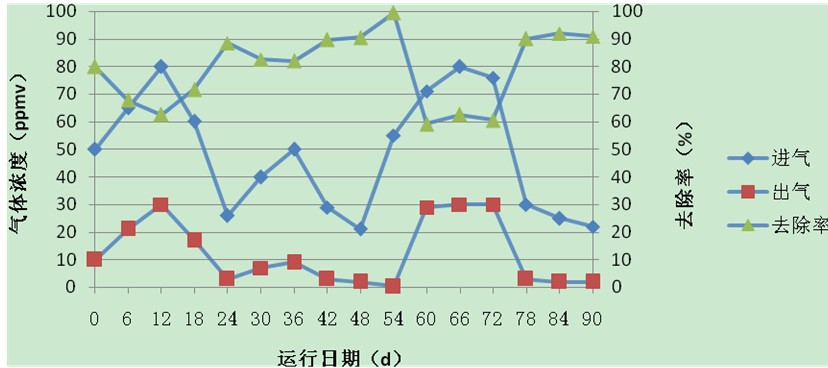
\includegraphics[width=150mm]{Img/fig1.jpg}
    \captionof{figure}{原水水质波动曲线}
    \label{fig1}
}
由图\ref{fig1}可以看出,试验期间,取得的焦化进水水质波动非常大,4月10日下午排入的焦化废水从71mg/L飙升至1422.23mg/L。完全超出了实验装置的进水标准。在波动渐渐平息后,废水进入一段稳定时期,原水COD在150左右波动。但是仍仍有逐步涨高的趋势,如图\ref{fig1}所示,22日水质突然上升至779mg/L。远超普通水质。\par
经现场观察,焦化厂废水因生产工艺不同可分为三类,包括黑色、白色和无色透明。其中白色及无色透明类离子浓度高,黑色废水中含有大量煤泥,以悬浮物为主要去除目标。\par
\subsection{不同水质来源的Fenton处理效果}
因废水水质波动问题,我们选取从拉水车的水单独处理,逐个排查每种水质的降解难易程度。具体实验结果如下:\par
\captionof{table}{不同水质的Fenton+混凝后的出水结果}
\label{tab2}
\begin{center}
\begin{tabular}{| c | c | c | c | c | c | c | c |}
    \hline
    编号 & 性状 & 双氧水ml & 硫酸亚铁g &  PAMml & 原水COD & 出水COD & 混凝COD\\ \hline 
    1 & 黑水 & 0.2 & 0.075 & 1 & 135.15 & 155.14 & 99.16\\ \hline 
    2 & 黑水 & 0.2 & 0.112 & 1 & 134.52 & 144.34 &  75.21\\ \hline 
    3 & 白水 & 0.2 & 0.112 & 1 & 97.96 & 63.17 & 6\\ \hline 
    4 & 白水 & 0.3 & 0.168 & 1 & 95.12 & 65.97 &  12\\ \hline 
    5 & 透明 & 0.2 & 0.112 & 1 & 105.96 & 119.15 & NA\\ \hline 
    6 & 透明 & 0.3 & 0.112 & 1 & 101.5 & 175.13 & NA\\ \hline 
\end{tabular}
\end{center}
\setlength{\parindent}{2em}
\par
以上实验结果证实,白色水质,经Fenton处理后,COD反而增加,经混凝后基本达标。黑色水质Fenton处理后同样上涨,混凝后COD降至100以下;透明水质因悬浮物含量极少,也出现上涨情况。其中混凝投加剂量为黑水(PAC100mg/L,PAM1mg/L),白水(PAC50mg/L,PAM1mg/L)。混凝后各种出水色度基本一致,透明澄清。\par
\subsection{改变Fenton反应pH值的实验结果}
后期改变Fenton反应的控制条件,发现反应pH对Fenton反应有较大影响,具体操作条件及实验结果如下:以黑色废水作为研究对象,芬顿试剂用量以各试剂与废水COD比值进行计算,如ρH2O2:ρCOD=1、2、3、4等计算。亚铁以ρFe$^{2+}$:ρCOD=0.2等。计COD=200mg/L。反应时间1h。\par
\begin{center}
\captionof{table}{pH值对Fenton反应的出水效果的影响}
\label{tab3}
\begin{tabular}{| c | c | c | c |}
    \hline
    编号 & pH值 & 双氧水ml & fenton出水COD\\ \hline 
    1 & 7 & 0.4 & 226.8\\ \hline 
    2 & 7 & 0.3 & 158.8\\ \hline 
    3 & 7 & 0.2 & 162.8\\ \hline 
    4 & 3 & 0.3 & 236.8\\ \hline 
    5 & 5 & 0.3 & 173.2\\ \hline     
\end{tabular}
\end{center}
\setlength{\parindent}{2em}
{
    \centering 
    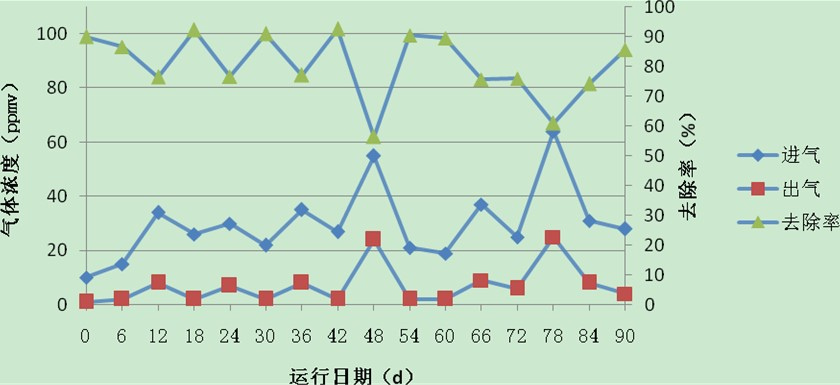
\includegraphics[width=150mm]{Img/fig2.jpg}
    \captionof{figure}{双氧水投加量的影响}
    \label{fig2}
}
反应中1、2、3组反应前不调pH,pH为7.5-8。第4组调pH至3,第5组调pH至4.7。反应后调PH至7。其中前三组仅加入2~4滴液碱。此处考察PH的影响,见2/4/5三组;以及双氧水投加量的影响,见1/2/3组。因此,最佳条件是双氧水投加量为0.3ml,PH为7时较好,即不需投加酸改变废水pH值,直接反应即可。\par
\subsection{改变Fenton试剂投加量的影响}
经上述实验后验证,Fenton反应前不需调节废水pH值,对该水质有一定处理效果,反应以白水为研究对象,硫酸亚铁控制在150mg/L,PAM 2mg/L,反应时间2h,继续调整Fenton试剂的投加量,具体实验结果及操作条件如下表:\par
\begin{center}
\captionof{table}{改变Fenton试剂投加量对出水结果的影响}
\label{tab4}
\begin{tabular}{| c | c | c | c | c |}
    \hline
    编号 & 双氧水ml & 碱用量ml & 原水COD & fenton出水COD\\ \hline 
    1 & 0.2 & 0.6 & 137.09 & 144.68\\ \hline 
    2 & 0.3 & 0.45 & 137.09 & 166.67\\ \hline 
    3 & 0.4 & 0.4 & 137.09 & 157.07\\ \hline 
    4 & 0.5 & 0.3 & 137.09 & 100.72\\ \hline 
    5 & 0.6 & 0.4 & 170.66 & 153.88\\ \hline 
    6 & 0.8 & 0.4 & 170.66 & 109.91\\ \hline 
    7 & 1 & 0.3 & 170.66 & 143.88\\ \hline 
\end{tabular}
\end{center}
\setlength{\parindent}{2em}
\par
在硫酸亚铁投加量一定的条件下,逐渐增加双氧水的投加量,出水COD值逐渐降低,继续提高加药量对出水结果无正面影响。本实验中,前后两组实验所用水质相同,但检测原水值有差异,此时有两个峰值点即1ml/L和1.6ml/L,为确保出水效果稳定,因此确定该类废水中双氧水投加量为1.6ml/L。\par
\subsection{水质中所含的氯离子浓度影响情况}
由上述结果可见,在不调节酸碱度的情况下,反涨现象有所下降,但仍与常规芬顿法处理后,废水中COD大幅下降有差别。因出水结果一直处于异常的不降反升的态势,我们随机检测了几组进水水样及5月20日当天试验装置的进出水水质情况。几乎所有水质中氯离子浓度全部超过一千,因而出水检测结果波动非常大。水质化验前,化验方法按照常规化验,未进行特别处理,因此所测COD值包含了氯离子被氧化所产生的COD值。\par 
经实际检测,原水中COD居高不下的原因是因为检测过程中未考虑氯离子对检测结果的影响。因此类废水属高盐低COD废水(氯离子高于1000,COD低于50)可采用低浓度测定法,消除氯离子的影响。正常检测后出水结果如下表所示:
\begin{center}
\captionof{table}{试验设备正常出水数据}
\label{tab5}
\begin{tabular}{| c | c | c | c | c |}
    \hline
    双氧水(ml) & 硫酸亚铁(g) & 氯离子(mg/L) & PAM(mg/L) & COD出水(mg/L)\\ \hline 
    0.8 & 0.1 & 2586.43 & 2 & 24.78\\ \hline     
\end{tabular}
\end{center}
\setlength{\parindent}{2em}
\par
由此说明,试验出水水质满足当地排放标准。在不加酸碱的情况下,投加Fenton试剂,可以对水中所含的重金属以及还原性物质如硫化物等进行沉淀,当水中有机性COD升高的情况下,再进行调节废水pH值进行反应。\par